%-------------------------------------------------------------------------------
% TEMPLATE FOR UCL MSc ECONOMICS THESES
% (c) Elliott Christensen, 2023

% This is a template for a MSc Thesis document based upon a template uploaded by Sofia Feist, 2020.
%------------------------------------------------------------------------------- 





% ------------------ DOCUMENT SETUP ------------------ 
% The document class defines the document type (article) and sets the font size (12pt)
\documentclass[12pt]{article}

% Your name
\author{the author}

% Inputs the Document Packages
\input{Packages}

% Controls how many subsections the document can take
%  and how many of those will get put into the contents pages.
%\setcounter{secnumdepth}{2}
% \setcounter{tocdepth}{2}

% Line Spacing
\setstretch{1.5}

% The folder path where the images will be uploaded
\graphicspath{ {./Image/} } 

% Places a dot after Chapter/Section/Subsection number in Table of Contents
% \renewcommand{\cftchapaftersnum}{.}
\renewcommand{\cftsecaftersnum}{.}
\renewcommand{\cftsubsecaftersnum}{}

%  Customize Dot spacing in Table of Contents/List of Figures/Tables
\renewcommand{\cftdotsep}{0.3}

% Numeration Type for Chapters and Sections (Roman I, II, II / Arabic 1, 2, 3)
% \renewcommand\thechapter{\Roman{chapter}}
\renewcommand\thesection{\arabic{section}}

% Line Break Properties
\tolerance=1
\emergencystretch=\maxdimen
\hyphenpenalty=10000
\hbadness=10000


% Formatting Table of Contents/Lists titles
\renewcommand{\contentsname}{\normalfont\bfseries\LARGE{CONTENTS}}
\renewcommand{\listfigurename}{\normalfont\bfseries\LARGE{LIST OF FIGURES}}
\renewcommand{\listtablename}{\normalfont\bfseries\LARGE{LIST OF TABLES}}


% Title Formatting customization
\titleformat{\chapter}{\normalfont\bfseries\LARGE}{\thechapter.}{1em}{\MakeUppercase}
\titlespacing*{\chapter} {0pt} {0pt} {0pt} % left, before, after

\titleformat{\section}{\normalfont\bfseries}{\thesection.}{1em}{\MakeUppercase}
\titlespacing*{\section} {0pt} {0pt} {0pt}

\titleformat{\subsection}{\normalfont\bfseries}{\thesubsection}{1em}{}
\titlespacing*{\subsection} {0pt} {10pt} {10pt}

\titleformat{\subsubsection}{\normalfont\bfseries}{}{1em}{}
\titlespacing*{\subsubsection} {0pt} {10pt} {10pt}


% HEADER AND FOOTER
\pagestyle{fancy}  % Set Page Style (Header and Footer Style)
\fancyhf{}  % Clears the header and footer (from the default info)

% Add a horizontal line by removing the % sign before the renewcommand (or vice versa): 
\renewcommand{\headrulewidth}{0.1pt}

% Header
\fancyhead[L]{\textit{Gabriel Richard}}
\fancyhead[C]{\textit{MSc Economics}}
\fancyhead[R]{\textit{September 2023}}

% Footer
\fancyfoot[C]{\thepage} % Page Number

% Change figure numbering per section
\numberwithin{figure}{section}
\numberwithin{table}{section}




%  -------------------------------------------------
%  --------- The document starts from here --------- 
%  -------------------------------------------------

\begin{document}
% ------------------  TITLE PAGE -------------------
\begin{titlepage}
\begin{center}
    % LSE LOGO
    \vspace*{1cm} % Adjust top spacing as needed
    \includegraphics[width=0.4\textwidth]{Image/LSE_logo.png} 
    
    \vfill % Elastic empty space filler
    
    % Title
    {\LARGE\textbf{The Direct Effect of the 2018 Trade War on Local Innovation:\\
    % Subtitle
    A Reduced-Form Shift-Share Approach\\}}

    \vspace{0.8cm}
    by\\
    \vspace{0.8cm}

    % Author
    {\LARGE\textbf{Gabriel Richard\\}}
    % Date
    \vspace{1.5cm}
    {\Large\textbf{May 2026}}

    \vfill

    \textbf{\setstretch{2.0} 
    Dissertation Supervisor: Xavier Jaravel\\
    \vspace{1cm}
    Dissertation submitted in part fulfilment of the\\
    Degree of Master of Science in Economics\\
    \vspace{1cm}
    Department of Economics\\
    London School of Economcis and Political Science\\}

    \vspace{2cm}
\end{center}
\end{titlepage}
% -------------------  Declaration  ---------------------


% ------------------  TABLE OF CONTENTS --------------------
\tableofcontents 



% -------------------  LIST OF FIGURES --------------------
%\newpage 
%{\let\oldnumberline\numberline       % Uncomment to add the word 'Figure' to figure number in List of Figures
%\renewcommand{\numberline}{\figurename~\oldnumberline}  
%\listoffigures%}
%\addcontentsline{toc}{section}{List of Figures} % Add List of figures into contents without any numeration 



% -------------------  LIST OF TABLES ---------------------
%\newpage
%\listoftables 
%\addcontentsline{toc}{section}{List of Tables} % Add List of tables into contents without any numeration 



% -----------------  ACKNOWLEDGEMENTS  -------------------
%\newpage
%\section*{Acknowledgements}
%\addcontentsline{toc}{section}{Acknowledgement}
%\blindtext 



% ----------------------  ABSTRACT -----------------------
\newpage
\section*{Abstract} % the Asterix (*) indicates that this section will be added to the table of contents but no number will be present beside it.
\addcontentsline{toc}{section}{Abstract}
This paper estimates the policy impact of the 2018 United States trade war on local innovation, measured by regional patenting rates. Because the highly discriminatory 2018 tariffs induced massive trade diversion, statutory tariffs are weak predictors of aggregate sector-level import changes. Consequently, this study employs a reduced-form IV shift-share regression that combines industry-level statutory tariff shocks with lagged county-level employment shares. To approximate a shock-level experimental ideal, the empirical strategy incorporates unit-level controls, alongside an incomplete share control to isolate quasi-experimental variation strictly within the tradable sector. Furthermore, controls for pre-2018 markups and structural production characteristics are introduced to correct for baseline imbalances and achieve conditional quasi-random assignment. To account for the mechanical correlation of unobserved errors between regions with similar industrial structures, the model is estimated using the mathematically equivalent shock-level regression. This yields exposure-robust standard errors clustered at the 3-digit NAICS level, supplemented by null-imposed confidence intervals. The results demonstrate that neither U.S. statutory output protection nor foreign retaliatory tariff assignments had a statistically detectable impact on short-term local innovation. Falsification tests using pre-trade-war patenting and historical trade flows confirm the validity of the design. However, because the reported confidence intervals accommodate economically substantial shifts, these findings are framed as a failure to detect a significant short-run response rather than definitive proof that innovation incentives were completely unchanged. Ultimately, these findings indicate that the sudden statutory assignment of the 2018 tariffs did not provide a causal signal sufficient to move the multi-year R\&D plans of U.S. firms.


\textbf{Keywords:} Microeconomics, Macroeconomics, Econometrics, Shift-Share, Instrument Variable




% ------------------  section START  --------------------


% -------------------  INTRODUCTION  ---------------------
\newpage
\section{Introduction} 
The year 2018 marked a historic change from decades of U.S. trade liberalization, as the United States enacted unilateral tariff increases on \$303 billion of annual U.S. imports. This return to protectionism escalated into a global trade war, pushing major trading partners, including China, the European Union, Canada, and Mexico, to impose retaliatory tariffs on \$127 billion of U.S. exports.  While the short-run price and welfare effects of these tariffs have been closely studied in the literature, their localized impact on technological innovation remains an open question. This paper asks: What was the direct effect of the 2018 trade war on local U.S. innovation? To answer this, I evaluate the impact of local county-level exposure to the 2018 tariff shocks on changes in regional patenting rates. \newline
Estimating the local impacts of trade policy is frequently complicated because of endogeneity, as unobserved local macroeconomic trends may simultaneously drive both actual trade flows and regional innovation. To address this, I rely on the shift-share econometric framework developed by \cite{BHJ2022} , which derives identification strictly from the quasi-random assignment of industry-level shocks rather than endogenous local exposure shares. \newline 
I employ a reduced-form shift-share regression rather than a traditional Two-Stage Least Squares Instrumental Variable design. In a standard 2SLS shift-share design, statutory tariff shocks would be used as an instrument to predict a separate endogenous treatment variable, such as the actual change in local import penetration. However, as demonstrated by \cite{Fajgelbaum2020}, the highly discriminatory 2018 tariffs induced trade diversion. Because U.S. firms heavily diverted their purchases to untargeted countries within the same broad sectors, the statutory tariffs are weak predictors of overall sector-level import changes. A reduced form approach shifts the question from estimating the effect of lost aggregate imports to estimating the intent-to-treat effect, allowing me to evaluate the direct policy impact of the statutory tariff shocks on local innovation. \newline
To ensure the validity of this research design, this paper approximates a shock-level experimental ideal. I introduce unit-level controls to absorb the electoral targeting of the U.S. tariffs, and incomplete share controls to account for the fact that tariffs exclusively targeted tradable sectors. Furthermore, falsification tests reveal the necessity of including shock-level controls, such as pre-2018 markups, to correct for baseline industry imbalances and achieve conditional quasi-random assignment. \newline
Finally, because shift-share designs suffer from exposure clustering, where regions with similar industrial structures have mechanically correlated errors, conventional regional standard errors are invalid. Following \cite{BHJ2022}, I use the mathematical equivalence of shift-share estimators to run the regression directly at the shock level. This allows to compute exposure-robust standard errors, that I cluster at the 3-digit NAICS level. 
My baseline estimates indicate that the 2018 trade war did not produce a statistically detectable effect on short-run regional innovation. Rather than proving that local R\&D incentives remained entirely static, the data simply lack the precision to rule out all economically meaningful shifts in patenting. Furthermore, falsification tests using historical trade and patenting trends confirm these findings are not driven by pre-existing trajectories. Taken together, these results imply that the chaotic, sudden nature of the 2018 statutory tariff assignments failed to generate a measurable causal disruption to the deeply entrenched, multi-year innovation pipelines of U.S. firms.

This paper contributes to three strands of economic literature. First, it adds a new dimension to the contemporary literature analyzing the 2018 U.S. trade war. While studies such as \cite{Amiti2019} and \cite{Fajgelbaum2020} demonstrate that the trade war resulted in trade diversion and complete tariff pass-through to domestic prices, this paper explores the implications of those coping mechanisms for local innovation. I demonstrate that the localized incentive to innovate remained statistically indistinguishable from its pre-war trend, a finding that is consistent with the hypothesis that firms redirected costs to consumers rather than altering their R\&D pipelines. Second, this paper contrasts with traditional models of trade-induced innovation, such as \cite{Bloom2011}, which posit that severe trade shocks force firms to upgrade technology to survive. I demonstrate that the statutory assignment of short-term tariffs characterized by extreme policy uncertainty behaves differently than structural market shifts. Finally, this paper contributes to the broader literature on local labor market responses to trade. Unlike the persistent, multi-decade structural shifts of the "China Shock" documented by \cite{ADH2013}, this study highlights the severe limitations of sudden, politically targeted trade policy as a viable causal instrument for domestic industrial upgrading.


% -------------------------------------------
% Simple image insert
%\begin{figure}[H] %[H] "corresponds to start the figure Here" 
%    \centering %alignment can be flushleft, centering or flushright
    %includegraphics is the command to include graphics or pictures, [Width should be defined with respect to textwidth]{The path/ location of the image in the specified folder}, the image should be either in .png, .jpg, .pdf formats faster processing
%    \includegraphics[width=0.5\textwidth]{Image/ucl_logo.png} 
%    \caption[The caption that goes into the list of figures]{\textit{\textbf{The image caption:}} Extended details about the image a.k.a legend}
%    \label{name the figures for cross reference}
%\end{figure}
% -------------------------------------------



% \cite{benner_2003} % Citation


% -------------------------------------------
% Image with multiple captions
%\begin{figure}[H]
%    \begin{flushleft}
%    \begin{subfigure}[b]{0.5\textwidth}
%    \includegraphics[width=\textwidth]{Image/ucl_logo.png}
%    \caption{write the caption}\label{fig:subfig1}
%    \end{subfigure}
%    \end{flushleft}
%        \hfill
%\begin{subfigure}[b]{0.5\textwidth}
%    \begin{flushright}
%    \includegraphics[width=\textwidth]{Image/ucl_logo.png}
%    \caption{write the caption}
%    \label{fig:subfig2}
%    \end{flushright}
%\end{subfigure}
%    \caption[The caption that goes into the list of figures]{\textbf{\textit{The image caption:}}Extended details about the image a.k.a legend}
%    \label{fig:Gel Extaction}
%\end{figure}
% -------------------------------------------


%\noindent \blindtext 


% -------------------------------------------
% Table (created with a table generator, e.g. https://www.tablesgenerator.com/# )
%\begin{table}[H]
%\caption[The caption that goes into the list of tables]{Generic Table}
%\label{tab:name the table for cross reference}
%\centering
%\begin{tabular}{lllll}
%\cline{1-3}
%\multicolumn{1}{|c|}{\cellcolor[HTML]{C0C0C0}\textbf{Header 1}} & \multicolumn{1}{c|}{\cellcolor[HTML]{C0C0C0}\textbf{Header 2}} & \multicolumn{1}{c|}{\cellcolor[HTML]{C0C0C0}\textbf{Header 3}} &  &  \\ \cline{1-3}
%\multicolumn{1}{|l|}{Content}                                   & \multicolumn{1}{l|}{Content}                                   & \multicolumn{1}{l|}{Content}                                   &  &  \\ \cline{1-3}
%\multicolumn{1}{|l|}{Content}                                   & \multicolumn{1}{l|}{Content}                                   & \multicolumn{1}{l|}{Content}                                   &  &  \\ \cline{1-3}
     
% -------------------------------------------

 % Section/Chapter entries can be done in the Main.tex file or in a  
                       % separate tex file for longer and more complex documents




% ---------------  REST OF THE DOCUMENT -----------------
\newpage
\section{Data and Descriptive Statistics}
\subsection{Data sources}

To measure local innovation, this study uses patent data from the United States Patent and Trademark Office. To accurately capture the timing of the innovation response, patents are strictly assigned based on their application date rather than their grant date, which is subject to severe administrative lags. Furthermore, to capture where the R\&D actually took place rather than where the corporate assignee is headquartered, patents are mapped to their U.S. county of origin based on the inventor's location. This dataset provides a granular record of total patent applications originating from each local labor market.

The exogenous shocks used are derived from the 2018 Trump statutory tariff as computed by \cite{Fajgelbaum2020} at the 6-digit NAICS level. To construct these measures, the authors mapped the specific product-level tariff changes announced by both the U.S. and foreign governments onto NAICS based on the 2017 import and export baskets.

To isolate the causal effect of the trade war from overlapping domestic trends, the model incorporates county-level demographic and political controls. The dataset integrates 2016 GOP presidential vote shares, local college attainment rates, baseline unemployment, and pre-existing manufacturing concentration at the FIPS code level, taken from \cite{Fajgelbaum2020} replication package.

To compute the exposure shares, I took the data from the County Business Patterns dataset. Raw CBP files are highly incomplete because the US Census Bureau suppresses employment counts for the majority of county-industry cells to preserve firm confidentiality. Therefore, to accurately construct the local exposure shares, I used the \cite{Eckert2020} algorithm. The algorithm uses a linear programming method that exploits the geographic and industrial adding-up constraints implicit in the Census data to accurately impute these suppressed missing values.

Finally, the dataset integrates baseline structural characteristics from the NBER-CES Manufacturing Industry Database and corporate markup matrices to satisfy the conditional exogeneity assumption.

\subsection{County-level manipulation and share-aggregation}

To measure the impact of the trade shocks on local innovation, the dependent variable is constructed as the change in patents per 100,000 residents rather than raw patent counts. Specifically, the difference in the number of patents filed before and after the shock—defined as the change between the pre-period (2014–2017) and the post-period (2018–2023)—is scaled by the 2016 county population. Utilizing a five-year post-shock window helps accommodate the natural lag between policy implementation, R\&D adjustment, and patent application. This scaling is necessary to isolate true changes in local innovation density, preventing the regression results from mechanically capturing baseline population size differences across counties (\cite{Chetty2019}).

Regional exposure shares are computed with the 2016 CBP data, imputed via the \cite{Eckert2020} imputation algorithm to resolve data suppression. The share for each 6-digit NAICS industry is calculated by taking its 2016 employment count in a given county and dividing it by the county's total 2016 employment. These shares are deliberately lagged to the beginning of the natural experiment. This ensures that local employment compositions are predetermined and structurally isolated from the 2018 trade war, preventing the tariff shocks from simultaneously altering the exposure shares themselves.

I then merged scaled patent changes via FIPS codes with a vector of 2016 unit-level controls, including the GOP presidential vote share (and its square), manufacturing employment share, college education share, and unemployment rate.

Because these regional confounders exist in geographic space while the tariff shock exists in industry space, they are projected to the NAICS level using the \cite{BHJ2022} shift-share aggregation framework. This allows to compute valid exposure-robust standard errors and avoid the mechanical correlation of residuals across regions with similar industries. I use the ssaggregate package to transition from a regional regression to the mathematically equivalent shock-level regression

\subsection{Industry-level controls}

To satisfy the \cite{BHJ2022} assumption of conditional quasi-random assignment, I calculated baseline industry characteristics from the NBER-CES database: production workers' share, capital to value-added ratio, log real wage, and equipment share, along with pre-2018 markups.

My final dataset was generated by merging the share-aggregated regional outcomes and unit-level controls with these specific industry-level controls and the 6-digit NAICS tariff shocks. This final dataset isolates the quasi-experimental variation strictly within the $333$ tradable manufacturing sectors, droping the non-tradable sectors, providing the shock-level framework required to run the final regression.

\subsection{Descriptive statistics}

The validity of the shift-share identification strategy relies on the presence of sufficient variation and dispersion in the industry-level tariff shocks. Descriptive analysis of the 2018 statutory shocks reveals significant heterogeneity across the manufacturing industries, with protective U.S. tariffs and foreign retaliatory tariffs - which refer to the aggregate retaliations from the six trading partners identified by \cite{Fajgelbaum2020}: China, Canada, Mexico, the EU, Russia, and Turkey - targeting distinct sectors of the economy. Summary statistics indicate that while many industries experienced a zero or near-zero baseline shock, a substantial subset of sectors faced sudden tariff increases exceeding 25\%, providing the necessary treatment variation required to identify an innovation response.

To verify that the model's statistical power is not driven by a few dominant industries, I computed the Inverse Herfindahl-Hirschman Index of the shock importance weights. In a shift-share design, the "effective number of shocks" is often much smaller than the raw count of industries; if a few large industries (like automotive or steel) carry all the weight, the standard asymptotic assumptions for the standard errors will fail. By calculating $1/HHI \approx 137.15$, I show that the effective sample size of the shocks is sufficiently large to satisfy the asymptotic requirements of \cite{BHJ2022}. This high effective count ensures that the standard errors are not artificially deflated by industry concentration and that the resulting confidence intervals, including the null-imposed intervals, are robust and reliable.

\begin{table}[!htbp] \centering
  \caption{Descriptive Statistics}
  \label{tab:descriptive_stats}
\begin{tabular}{lcccc}
\hline \hline
 & Mean & Std. Dev. & Min & Max \\
\hline
\multicolumn{5}{l}{\textit{Panel A: Industry level (N = 333, effective N = 1/HHI = 137.15)}} \\
U.S. Tariff Shock ($T_0$) & 0.0216 & 0.0233 & 0.0000 & 0.1437 \\
Retaliation Shock ($R_0$) & 0.0100 & 0.0158 & 0.0000 & 0.1342 \\
Markups & 1.6068 & 0.2560 & 1.3800 & 1.9400 \\
Production Worker Share & 0.6861 & 0.1215 & 0.3016 & 0.9028 \\
Capital / Value Added & 1.0221 & 1.1581 & 0.1825 & 17.4791 \\
Log Real Wage & 10.9502 & 0.3223 & 10.2184 & 13.0360 \\
Equipment Share & 0.6663 & 0.1077 & 0.2390 & 0.9001 \\
\hline
\multicolumn{5}{l}{\textit{Panel B: County level (N = 3145)}} \\
Manufacturing Share (2016) & 0.1221 & 0.1090 & 0.0000 & 0.6891 \\
GOP Vote Share (2016) & 0.6671 & 0.1611 & 0.0425 & 0.9675 \\
College Share (2016) & 13.5758 & 5.5248 & 1.7000 & 43.0000 \\
\hline \hline
\end{tabular}
\end{table}


% -----------------------------------------------------------------
% Vertically Stacked Regional Tariff Exposure Heat Maps
% -----------------------------------------------------------------
\begin{figure}[!htbp]
    \centering
    % Top Panel: Protective Tariffs
    \begin{subfigure}[b]{0.95\textwidth}
        \centering
        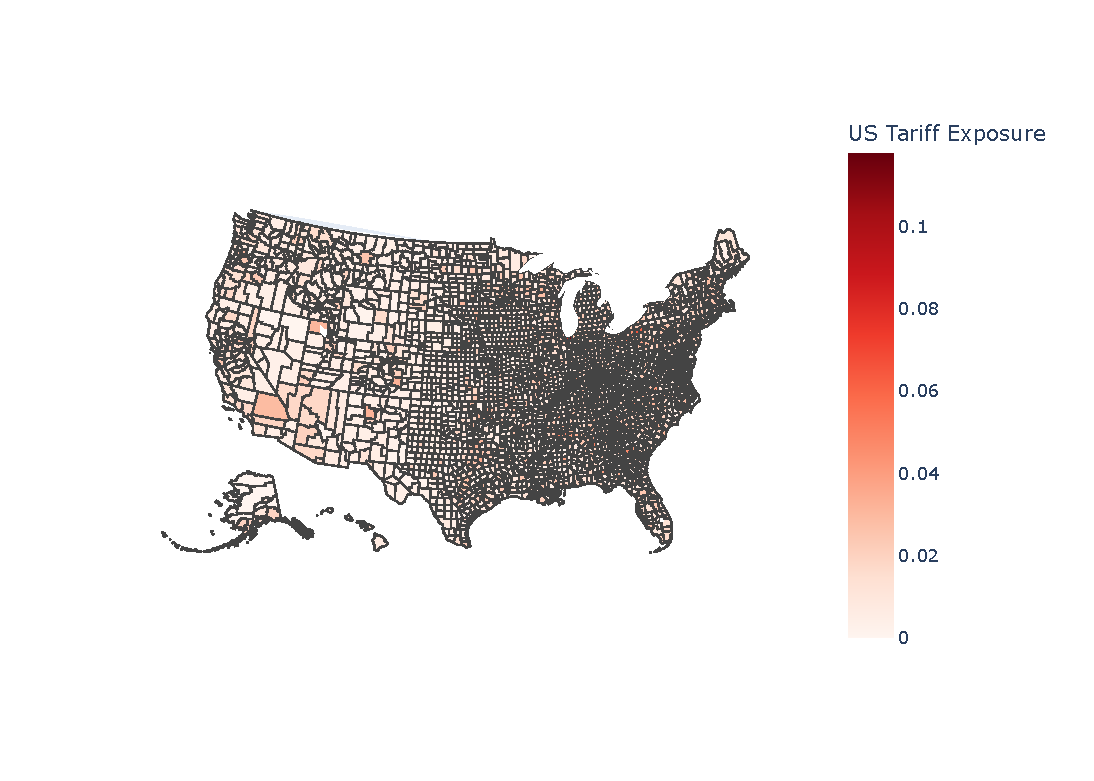
\includegraphics[width=\textwidth]{../outputs/figures/map_protective.pdf}
        \caption{U.S. Protective Tariffs}
        \label{fig:map_protective}
    \end{subfigure}
    
    \vspace{0.5cm} % Adds a clean vertical gap between the two panels
    
    % Bottom Panel: Retaliatory Tariffs
    \begin{subfigure}[b]{0.95\textwidth}
        \centering
        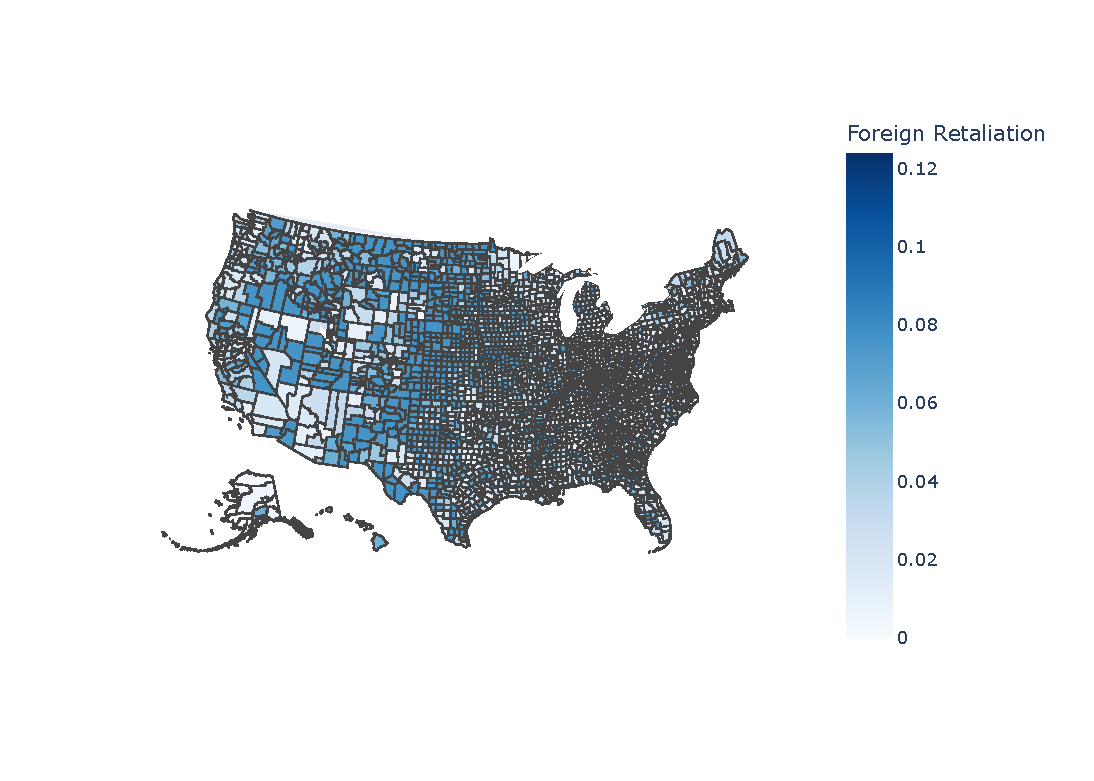
\includegraphics[width=\textwidth]{../outputs/figures/map_retaliatory.pdf}
        \caption{Foreign Retaliatory Tariffs}
        \label{fig:map_retaliatory}
    \end{subfigure}
    
    \caption{Geographic Variation in 2018 Tariff Exposure}
    \label{fig:stacked_maps}
    \vspace{0.2cm}
    
    \begin{minipage}{0.95\textwidth}
        \footnotesize \textit{Notes:} These maps illustrate the spatial distribution of trade war shocks across U.S. counties. Panel (a) highlights exposure to U.S. protective tariffs, concentrating intensely across the industrial Rust Belt. Panel (b) highlights regional exposure to foreign retaliatory measures, heavily hitting agricultural economies across the Midwestern plains.
    \end{minipage}
\end{figure}

\newpage
\section{Empirical Strategy}
\subsection{First Stage}

In a traditional Two-Stage Least Squares shift-share design, one would use the exogenous tariff shocks to predict a separate endogenous treatment variable, such as the actual change in local import volumes, before evaluating the effect on innovation.

Following the estimator equivalence result of \cite{BHJ2022}, we can evaluate this first-stage relationship directly at the shock level NAICS-6 to test if statutory tariffs significantly depressed aggregate industry imports. The industry-level first-stage regression is specified as:

$$ \Delta \ln M_n = \alpha + \lambda g_n + \gamma' q_n + \varepsilon_n $$

With $\Delta \ln M_n$: The change in aggregate U.S. import volumes for NAICS-6 industry $n$ between the 2017 pre-shock baseline and the 2019 post-shock period. To properly account for zero-trade flows without dropping data, this is calculated using the inverse hyperbolic sine transformation.
$g_n$: The 2018 statutory tariff shock applied to industry $n$.
$q_n$: The vector of share-aggregated unit-level controls. Because regional characteristics must be translated to the shock level, this vector includes the exposure-weighted averages of the 2016 county manufacturing share, the 2016 GOP presidential vote share and its square, the college education share, and the unemployment rate. The regression is weighted by the industry importance weights ($s_n$), with standard errors clustered at the 3-digit NAICS level to account for mutual correlation across related sectors.

Estimating this first-stage specification yields a coefficient on the statutory tariff shock of $\lambda = -1.007$ with a p-value of 0.117. This statistically insignificant result indicates that the 2018 statutory tariffs failed to meaningfully predict changes in total sector-level import volumes, rendering the statutory tariffs a weak instrument for actual aggregate trade flows. 

Economically, this null first stage is driven by a massive trade diversion effect. As demonstrated by \cite{Fajgelbaum2020}, the highly discriminatory nature of the 2018 U.S. tariffs caused imports of specifically targeted micro-varieties (country-product pairs, like Chinese steel) to plummet by an average of 31.7\%. However, because U.S. firms simply dodged these penalties by shifting their supply chains to untargeted countries within the same sector, the total volume of imports within targeted NAICS-6 sectors fell by a mere 0.2\%. Because the statutory tariff shocks operates at the broader NAICS-6 sector level, these micro-level supply chain disruptions completely wash out in the aggregate data.

This finding provides an empirical justification for abandoning a traditional 2SLS approach. Because massive trade diversion breaks the predictive link between statutory tariffs and overall sector-level import penetration, evaluating actual trade volumes is econometrically invalid here. Instead, I move to a reduced-form shift-share design, where local innovation is regressed directly on the statutory tariff shocks to identify the intent-to-treat direct policy effect of the 2018 trade war.

\begin{table}[!htbp] \centering
  \caption{First Stage: 2018 Tariffs and 2017--2019 Import Changes}
  \label{tab:first_stage}
\begin{tabular}{@{\extracolsep{5pt}}lc}
\\[-1.8ex]\hline
\hline \\[-1.8ex]
& \multicolumn{1}{c}{\textit{Dependent variable: $\Delta \ln$ imports, 2017--2019}} \
\cr \cline{2-2}
\\[-1.8ex] & (1) \\
\hline \\[-1.8ex]
 Capital / Value Added & -0.032$^{**}$ \\
& (0.013) \\
 Constant & -0.892$^{}$ \\
& (0.837) \\
 Equipment Share & 0.363$^{}$ \\
& (0.376) \\
 Log Real Wage & -0.036$^{}$ \\
& (0.088) \\
 Markups & -0.042$^{}$ \\
& (0.090) \\
 Production Worker Share & 0.130$^{}$ \\
& (0.192) \\
 U.S. Tariff Shock ($T_0$) & -1.007$^{}$ \\
& (0.643) \\
\hline \\[-1.8ex]
 Observations & 333 \\
 $R^2$ & 0.020 \\
 Adjusted $R^2$ & 0.002 \\
 Residual Std. Error & 0.415 (df=326) \\
 F Statistic & 9.812$^{***}$ (df=6; 326) \\
\hline
\hline \\[-1.8ex]
\textit{Note:} & \multicolumn{1}{r}{$^{*}$p$<$0.1; $^{**}$p$<$0.05; $^{***}$p$<$0.01} \\
\end{tabular}
\end{table}
\newpage
\subsection{Shift-Share Design and Shock-Level Experimental Idea}

To estimate the causal effect of the 2018 trade war on local innovation, this paper uses a reduced-form shift-share econometric design that overcomes the endogeneity of local macroeconomic trends by exploiting the quasi-random assignment of industry-level tariffs. A standard OLS regression of regional patenting on local trade exposure is plagued by omitted variable bias, as unobserved local economic dynamics likely drive both regional innovation and actual trade outcomes. 

To circumvent this, I use the \cite{BHJ2022} IV shift-share framework. The instrument is constructed as:
$$ Z_i = \sum_n s_{in} g_n $$
where $g_n$ is the statutory tariff change in NAICS industry $n$, and $s_{in}$ is the pre-determined employment share of industry $n$ in county $i$. 

The validity of this shift-share strategy is motivated via a shock-level experimental ideal, where identification stems entirely from the quasi-random assignment of the industry-level tariff shocks rather than the endogenous local exposure shares. In this framework, one can imagine a hypothetical lottery that randomly assigns tariff shocks to different manufacturing industries. If  tariff assignments are as-good-as-random at the industry level, then any share-weighted average of these random subsidies is also as-good-as-randomly assigned at the regional level, mathematically guaranteeing that the instrument $Z_i$ is orthogonal to the unobserved residual $\varepsilon_i$. This logic holds regardless of whether the initial exposure shares $s_{in}$ are themselves endogenous. Thus the instrument bypasses the omitted variable bias.

Following the rejection of the first stage, I estimate the causal impact of trade policy using a reduced-form specification at the county level:
$$\Delta Y_i = \beta Z_i + \gamma W_i + \epsilon_i $$where $\Delta Y_i$ is the change in patents per 100,000 residents. In this framework, the coefficient of interest, $\beta$, identifies the Intent-to-Treat effect of statutory output protection assignment. This estimand measures the average change in local innovation density resulting from the application of tariffs to a county’s production mix. Therefore, the model captures the net impact of the policy announcement and legal application, incorporating subsequent firm-level adjustments such as trade diversion and price pass-through documented in the literature.


\subsection{Approximating the ideal with controls}

To approximate the experimental ideal and isolate the quasi-experimental variation in trade policy, the model incorporates county-level controls, which are aggregated to the industry level to absorb the confounding effects of electoral targeting and local macroeconomic conditions. As demonstrated by \cite{Fajgelbaum2020}, the 2018 U.S. protective tariffs exhibited an inverted-U shape with respect to the 2016 Republican presidential vote share, indicating deliberate targeting toward sectors concentrated in electorally competitive swing states (see Figure \ref{fig:political_targeting}). By contrast, foreign retaliatory tariffs heavily targeted agricultural sectors concentrated in Republican-leaning areas. To absorb this electoral confounding, alongside baseline local labor market dynamics, the model controls for the 2016 GOP presidential vote share, and its square, as well as the manufacturing share, college education share, and the unemployment rate in 2016. Because the main specification is estimated directly at the shock level across $333$ 6-digit NAICS tradable industries, these county-level controls are translated to the industry level via the $ssaggregate$ function, which computes the exposure-weighted average of these regional characteristics for each industry. This allows the local political and demographic confounders to be properly controlled in the shock-level regression.

% -----------------------------------------------------------------
% Political Targeting Fit (LOESS Curves for Empirical Justification)
% -----------------------------------------------------------------
\begin{figure}[!htbp]
    \centering
    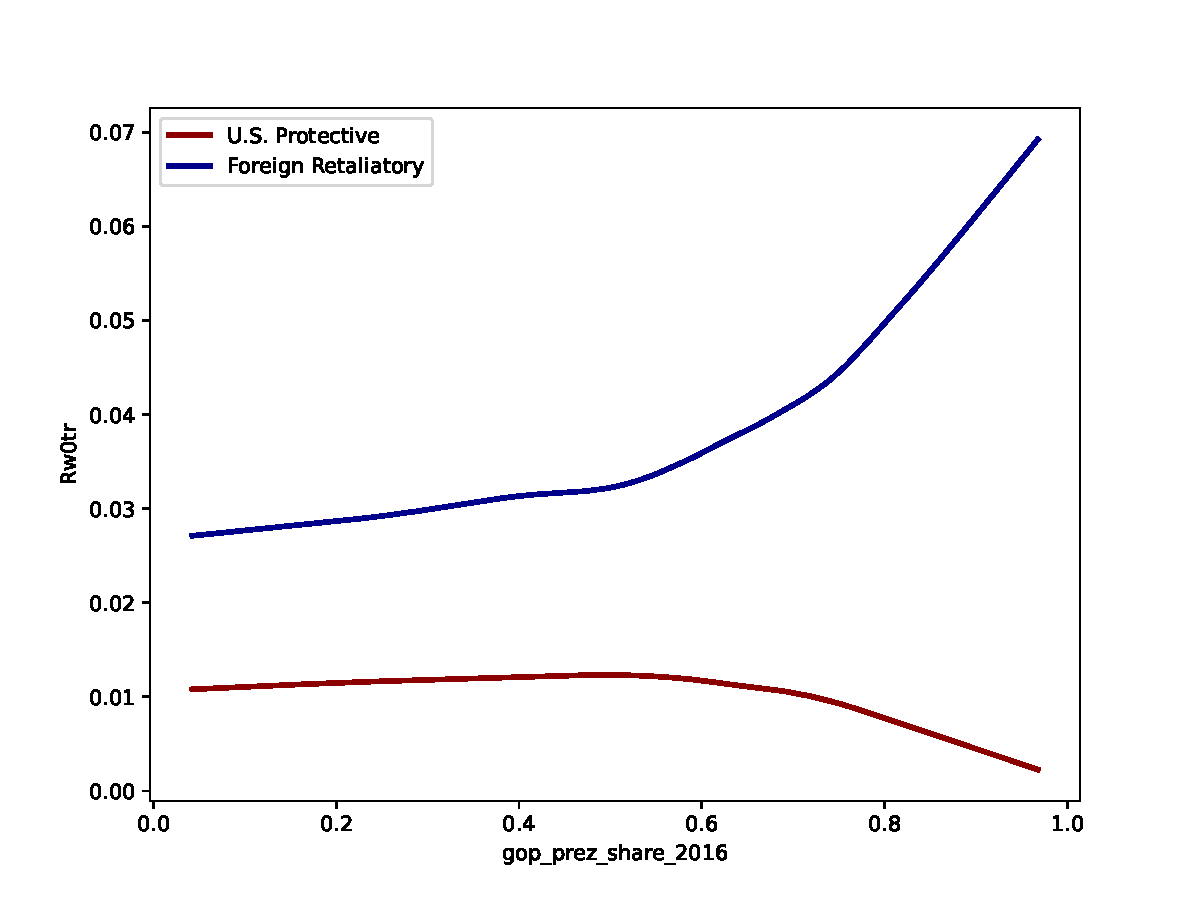
\includegraphics[width=0.85\textwidth]{../outputs/figures/political_targeting.pdf}
    \caption{Non-Parametric Fit of Tariff Exposure by 2016 GOP Vote Share}
    \label{fig:political_targeting}
    \vspace{0.2cm}
    
    \begin{minipage}{0.9\textwidth}
        \footnotesize \textit{Notes:} This figure presents a non-parametric LOESS smoothing fit plotting county-level tariff exposure against the 2016 Republican presidential vote share, weighted by county population. The dark red curve maps exposure to U.S. protective tariffs, illustrating a inverted-U shape that peaks in competitive swing counties (approximately 40--60\% GOP vote share). Conversely, the dark blue curve maps exposure to foreign retaliatory measures, displaying a monotonic upward slope that disproportionately targets reliable Republican strongholds. This asymmetry provides the empirical justification for explicitly controlling for both the linear and quadratic terms of the 2016 GOP presidential vote share in our baseline structural equations.
    \end{minipage}
\end{figure}
\newpage
Furthermore, the model directly incorporates industry-level controls to approach conditional quasi-random assignment, correcting for the fact that tariffs systematically targeted low-markup industries and ensuring balance across fundamental production characteristics. Shock-level falsification tests, conducted in accordance with the \cite{BHJ2022} framework, reveal that the 2018 statutory tariffs were unbalanced with respect to industry market power, measured via the markups. To isolate the residual quasi-experimental variation in the shocks, I include these baseline markups as a direct control. Additionally, even though they successfully passed the balance tests, I include other structural industry controls established by \cite{Acemoglu2016}. Specifically, the production worker share, the capital to value-added ratio, the logarithm of real wages, and the high-tech equipment share, to absorb broad trends in manufacturing. Because the estimating equation is already defined at the 6-digit NAICS shock level, these structural variables are simply included as direct covariates, ensuring the regression strictly leverages the conditionally exogenous variation in the 2018 tariffs.

Because the tariff shocks apply exclusively to the tradable manufacturing sector, the exposure shares do not sum to one. \cite{BHJ2022} show that when the sum of shares $S_i = \sum_n s_{in}$ varies across observations, the shift-share instrument mechanically correlates with $S_i$, violating quasi-random assignment. To mathematically correct this incomplete-share bias, the non-tradable sector is removed from the shock-level identifying variation, and the total county manufacturing employment share $S_i$ is included as a unit-level control in the regional covariate vector $W_i$ prior to residualization. By controlling for the sum of shares, the regression successfully isolates conditional quasi-random variation strictly among the manufacturing industries a county holds.

Finally, to compute exposure-robust standard errors and correct for the mechanical correlation of unobserved shocks across regions with similar industrial structures, the main specification is estimated via a mathematically equivalent shock-level regression. In shift-share designs, traditional regional standard errors are invalid because local labor markets with similar industry exposure shares have mechanically correlated unobserved residuals. As demonstrated by \cite{Adao2019}, failing to account for this exposure clustering leads to severe over-rejection of the null hypothesis. The \cite{BHJ2022} framework proves that the regional estimator $\beta$ from the baseline specification $\Delta Y_i = \beta Z_i + \gamma' W_i + \varepsilon_i$ is numerically equivalent to the coefficient obtained from an industry-level regression. To execute this equivalence, the unit-level controls $W_i$ (including the GOP vote share, unemployment, college education, and baseline manufacturing share) are first residualized from the regional outcomes. I use the $ssaggregate$ package to project these partialled-out regional outcomes into shock-level aggregates, denoted as $\bar{Y}_n^\perp$. Consequently, the inference is conducted via the equivalent shock-level WLS regression:
$$ \bar{Y}_n^\perp = \alpha + \beta g_n + \delta' q_n + \bar{\varepsilon}_n^\perp $$
where the regression is weighted by industry importance weights $s_n$ and includes the direct industry-level structural controls $q_n$. Because the unit-level political and demographic confounders are absorbed during the regional residualization step, they do not appear in the final shock-level estimating equation, leaving only the industry-level characteristics. By aggregating the regional data to the NAICS level, we can cluster the standard errors at the 3-digit NAICS level, ensuring the inference properly accounts for mutual correlation across related industries and remains asymptotically valid.

\newpage
\section{Main Results and Inference}
\subsection{The Role of Baseline Structural Confounders}

The baseline industry controls successfully partial out significant structural confounding trends in local innovation. As established in the empirical strategy, the following results are estimated via the equivalent shock-level regression across $333$ tradable industries, yielding exposure-robust standard errors clustered at the 3-digit NAICS level (21 clusters). Note that because the unit-level electoral and demographic controls were residualized prior to aggregation, Tables \ref{tab:main_regression} and \ref{tab:retaliation_regression} exclusively report the coefficients for the remaining industry-level structural covariates. As shown in both Table \ref{tab:main_regression} and Table \ref{tab:retaliation_regression}, baseline industry characteristics strongly predict regional patenting growth independent of the trade shocks. Pre-2018 markups maintain a positive and marginally significant effect ($\beta=7.491$, $p<0.1$ in Table 4.1), which can indicate that highly profitable sectors, with high markups, possess the excess capital necessary to fund R\&D. Furthermore, the inclusion of the \cite{Acemoglu2016} production controls reveals that local labor markets concentrated in capital-intensive sectors ($\beta=-5.075$, $p<0.01$) and high-tech equipment investment ($\beta=-19.362$, $p<0.05$) experienced slower patenting growth during this period, while regions heavily relying on production workers saw relative increases. By controlling for these variables, the shift-share design isolates the quasi-experimental variation in tariffs from these industry trends.

\subsection{The Null Effect of U.S. Protective Tariffs on Innovation}

Conditional on this set of industry controls, the reduced-form estimate reveals that U.S. protective tariffs had no significant short-term effect on local innovation. In Table \ref{tab:main_regression}, the coefficient on the U.S. statutory tariff shock is small and statistically indistinguishable from zero ($\beta = 3.125$, SE $= 42.233$). While the point estimate is near zero, the null-imposed 95\% confidence interval (Table \ref{tab:robust_cis}) is wide, spanning [-79.31,85.56]. This indicates that the current data can only reliably rule out extremely large innovation surges, as the upper bound of the interval remains compatible with economically meaningful shifts. Thus, the result can be framed as a failure to detect a significant short-run response rather than definitive proof that innovation incentives were completely static.

This finding contrasts with traditional theoretical predictions regarding trade and innovation, but aligns with the highly uncertain environment of the 2018 trade war. While literature such as \cite{Bloom2011} suggests that import competition induces firms to accelerate technological innovation to survive, one might expect the sudden removal of this competition via protective tariffs to negatively impact patenting. However, the 2018 tariffs were not a stable, long-term industrial policy. Both \cite{Amiti2019} and \cite{Fajgelbaum2020} demonstrate that these tariffs resulted in complete pass-through to domestic prices, abruptly raising intermediate input costs for U.S. firms and forcing billions of dollars in trade to be redirected to avoid the tariffs. Because the 2018 trade war was characterized by extreme policy uncertainty, and because innovation pipelines require multi-year investments, firms likely viewed the protective tariffs as temporary political noise rather than a structural shift warranting immediate R\&D acceleration, leaving their structural imperative to innovate largely unchanged.

\subsection{The Null Effect of Foreign Retaliatory Tariffs on Innovation}

Similarly, exposure to foreign retaliatory tariffs yields no statistically detectable short-run impact on local patenting, though wide confidence intervals preclude definitively ruling out theories of defensive innovation. Table \ref{tab:retaliation_regression} demonstrates that the coefficient on the retaliatory tariff shock is insignificant ($\beta=37.937$, SE $=33.638$). Theories of trade-induced innovation often posit that severe negative trade shocks can force firms into upgrading their technology to remain globally competitive. As established by \cite{Fajgelbaum2020}, the 2018 retaliatory tariffs were not economically optimized to target high-tech manufacturing, rather, they were deliberately engineered to target agricultural sectors concentrated in heavily Republican-leaning counties to inflict maximal political pain. Once these structural and geographic confounders are strictly controlled for in the shift-share design, the residual policy effect on innovation is null. The lack of a detectable innovation response to these retaliations is consistent with the operational adjustments documented in the broader 2018 trade war literature. While \cite{Fajgelbaum2020} estimate that retaliations caused a 9.9\% decline in targeted U.S. export values, this represented a sudden revenue loss driven by the trade war, but not a shift in global comparative advantage. Under the policy uncertainty, firms absorbed the sudden demand shock or redirected their supply chains instead of embarking on costly, high-risk patenting augmentation.

Ultimately, both the U.S. output protection and foreign retaliatory tariff results point to the same conclusion: the statutory assignment of the 2018 tariffs did not provide a statistically detectable causal signal sufficient to change the incentive to innovate of U.S. firms.


\begin{table}[!htbp] \centering
  \caption{U.S. Protective Tariffs and Local Innovation}
  \label{tab:main_regression}
\begin{tabular}{@{\extracolsep{5pt}}lc}
\\[-1.8ex]\hline
\hline \\[-1.8ex]
& \multicolumn{1}{c}{\textit{Dependent variable: Change in patents per 100k}} \
\cr \cline{2-2}
\\[-1.8ex] & (1) \\
\hline \\[-1.8ex]
 Capital / Value Added & -5.075$^{***}$ \\
& (1.517) \\
 Constant & -22.762$^{}$ \\
& (31.388) \\
 Equipment Share & -19.362$^{**}$ \\
& (9.127) \\
 Log Real Wage & 0.747$^{}$ \\
& (2.403) \\
 Markups & 7.491$^{*}$ \\
& (4.358) \\
 Production Worker Share & 28.203$^{***}$ \\
& (8.026) \\
 U.S. Tariff Shock ($T_0$) & 3.125$^{}$ \\
& (42.233) \\
\hline \\[-1.8ex]
 Observations & 333 \\
 $R^2$ & 0.102 \\
 Adjusted $R^2$ & 0.086 \\
 Residual Std. Error & 15.339 (df=326) \\
 F Statistic & 5.977$^{***}$ (df=6; 326) \\
\hline
\hline \\[-1.8ex]
\textit{Note:} & \multicolumn{1}{r}{$^{*}$p$<$0.1; $^{**}$p$<$0.05; $^{***}$p$<$0.01} \\
\end{tabular}
\end{table}
\begin{table}[!htbp] \centering
  \caption{Foreign Retaliatory Tariffs and Local Innovation}
  \label{tab:retaliation_regression}
\begin{tabular}{@{\extracolsep{5pt}}lc}
\\[-1.8ex]\hline
\hline \\[-1.8ex]
& \multicolumn{1}{c}{\textit{Dependent variable: Change in patents per 100k}} \
\cr \cline{2-2}
\\[-1.8ex] & (1) \\
\hline \\[-1.8ex]
 Capital / Value Added & -5.004$^{***}$ \\
& (1.517) \\
 Constant & -18.888$^{}$ \\
& (30.852) \\
 Equipment Share & -19.510$^{**}$ \\
& (8.959) \\
 Log Real Wage & 0.461$^{}$ \\
& (2.363) \\
 Markups & 7.607$^{*}$ \\
& (3.885) \\
 Production Worker Share & 26.342$^{***}$ \\
& (8.368) \\
 Retaliation Shock ($R_0$) & 37.937$^{}$ \\
& (33.638) \\
\hline \\[-1.8ex]
 Observations & 333 \\
 $R^2$ & 0.104 \\
 Adjusted $R^2$ & 0.088 \\
 Residual Std. Error & 15.311 (df=326) \\
 F Statistic & 5.690$^{***}$ (df=6; 326) \\
\hline
\hline \\[-1.8ex]
\textit{Note:} & \multicolumn{1}{r}{$^{*}$p$<$0.1; $^{**}$p$<$0.05; $^{***}$p$<$0.01} \\
\end{tabular}
\end{table}


\newpage
\section{Robustness and Falsification Tests}
\subsection{Pre-Trend Falsification Tests}

Falsification tests using historical pre-trends confirm that the 2018 tariffs were not implemented as a reaction to pre-existing, divergent trajectories in regional innovation or industry trade flows. To ensure the validity of the shift-share design, it is first necessary to rule out reverse causality. If the U.S. government systematically assigned higher tariffs to industries that were already experiencing an innovation downtrend or an import surge prior to 2018, the core identifying assumption of the natural experiment would be violated. By testing whether the 2018 statutory tariff shocks hold any explanatory power over historical patenting and trade dynamics from before the trade war, I can establish whether the tariffs act as a true, unanticipated shock rather than a mere continuation of prior macroeconomic trends.

Table \ref{tab:innovation_pretrend} estimates the baseline shock-level regression using the pre-trend change in regional patenting as the dependent variable. Conditional on the NBER-CES industry controls, the coefficient on the statutory tariff shock is insignificant. Because the statutory tariff shocks do not significantly predict historical patenting outcomes from the preceding years, this test successfully rules out the threat of reverse causality or policy endogeneity. It proves that the government did not deploy protective tariffs to specifically aid regions or industries that were already on an innovation downtrend prior to the trade war.

Further falsification tests on historical trade flows, demonstrate that the Trump administration did not disproportionately impose tariffs on industries that were already experiencing systematic import surges or price anomalies prior to 2018. Mirroring the robustness checks conducted by \cite{Fajgelbaum2020}, Table \ref{tab:trade_pretrends} tests for preexisting trade trends by regressing the 2013–2017 changes in import values (Column 1), import quantities (Column 2), and unit values or prices (Column 3) directly on the 2018 statutory tariff shocks. Across all three trade specifications, the tariff shock coefficients are small and statistically indistinguishable from zero. Furthermore, the regression models yield extremely low F-statistics and near-zero $R^2$ values, indicating that the 2018 tariff have no explanatory power over prior trade dynamics. These null results successfully replicate the findings in the existing trade literature, proving that the industries targeted during the trade war were not already on anomalous trade trajectories and proving the validity of the tariff shocks as a natural experiment.

\begin{table}[!htbp] \centering
  \caption{Pre-Trend Falsification: 2014--2017 Patenting}
  \label{tab:innovation_pretrend}
\begin{tabular}{@{\extracolsep{5pt}}lc}
\\[-1.8ex]\hline
\hline \\[-1.8ex]
& \multicolumn{1}{c}{\textit{Dependent variable: Change in patents per 100k, 2014--2017}} \
\cr \cline{2-2}
\\[-1.8ex] & (1) \\
\hline \\[-1.8ex]
 Capital / Value Added & 1.059$^{***}$ \\
& (0.351) \\
 Constant & -5.331$^{}$ \\
& (9.377) \\
 Equipment Share & -1.286$^{}$ \\
& (2.391) \\
 Log Real Wage & 0.316$^{}$ \\
& (0.803) \\
 Markups & -2.659$^{**}$ \\
& (1.035) \\
 Production Worker Share & 9.025$^{***}$ \\
& (3.261) \\
 U.S. Tariff Shock ($T_0$) & -4.867$^{}$ \\
& (9.373) \\
\hline \\[-1.8ex]
 Observations & 333 \\
 $R^2$ & 0.161 \\
 Adjusted $R^2$ & 0.145 \\
 Residual Std. Error & 3.469 (df=326) \\
 F Statistic & 4.042$^{***}$ (df=6; 326) \\
\hline
\hline \\[-1.8ex]
\textit{Note:} & \multicolumn{1}{r}{$^{*}$p$<$0.1; $^{**}$p$<$0.05; $^{***}$p$<$0.01} \\
\end{tabular}
\end{table}

\begin{table}[!htbp] \centering
  \caption{Pre-Trend Falsification: 2013--2017 Import Trends}
  \label{tab:trade_pretrends}
\begin{tabular}{@{\extracolsep{5pt}}lccc}
\\[-1.8ex]\hline
\hline \\[-1.8ex]
\\[-1.8ex] & \multicolumn{1}{c}{Import value} & \multicolumn{1}{c}{Import quantity} & \multicolumn{1}{c}{Unit value}  \\
\hline \\[-1.8ex]
 Constant & 0.002$^{}$ & 0.003$^{***}$ & -0.001$^{}$ \\
& (0.002) & (0.001) & (0.002) \\
 U.S. Tariff Shock ($T_0$) & 0.054$^{}$ & 0.021$^{}$ & 0.022$^{}$ \\
& (0.040) & (0.030) & (0.040) \\
\hline \\[-1.8ex]
 Observations & 361 & 361 & 361 \\
 $R^2$ & 0.007 & 0.001 & 0.001 \\
 Adjusted $R^2$ & 0.004 & -0.002 & -0.002 \\
 Residual Std. Error & 0.021 (df=359) & 0.036 (df=359) & 0.028 (df=359) \\
 F Statistic & 1.791$^{}$ (df=1; 359) & 0.482$^{}$ (df=1; 359) & 0.301$^{}$ (df=1; 359) \\
\hline
\hline \\[-1.8ex]
\textit{Note:} & \multicolumn{3}{r}{$^{*}$p$<$0.1; $^{**}$p$<$0.05; $^{***}$p$<$0.01} \\
\end{tabular}
\end{table}
\newpage
\subsection{Controls balance tests}

Shock-level balance tests reveal the structural targeting in the 2018 trade policy, identifying which baseline industry characteristics must be controlled for to achieve conditional quasi-random assignment. While pre-trend tests rule out reverse causality over time, the shift-share instrument must also be evaluated for cross-sectional balance. If the U.S. government systematically assigned higher protective tariffs to industries with inherently different production structures the exogeneity assumption is violated. Following \cite{BHJ2022}, I empirically evaluate this by regressing pre-existing industry-level characteristics directly on the tariff shocks, weighting by the industry importance weights and clustering standard errors appropriately. Testing whether the structure of employment and technology correlates with the 2018 tariffs allows us to pinpoint exact sources of policy endogeneity, thereby justifying the inclusion of the controls used in the main empirical specification.

The balance tests reveal that the U.S. government protected low-markup sectors while remaining structurally balanced across other fundamental manufacturing dimensions. Panel A of Table \ref{tab:balance_tests_stacked} shows that the balance test for baseline market power fails: the coefficient on markups is negative and statistically significant at the 5\% significance level. This result indicates that the 2018 tariffs were not unconditionally random, but rather were targeted to shield vulnerable, low-markup commodity sectors (such as basic steel or aluminum) that struggle with profitability and foreign competition. To cure this omitted variable bias, my empirical strategy partials out this confounder by controlling for markups, isolating the residual variation in the tariffs and satisfying the requirement for conditional quasi-random assignment.

Other falsification tests across standard production characteristics confirm that the 2018 U.S. tariffs were otherwise structurally balanced. As shown in Panel B of Table \ref{tab:balance_tests_stacked}, regressing the 2018 statutory tariff shocks on 2016 industry characteristics, specifically labor intensity, capital intensity, real wages, and the share of high-tech equipment investment, yields insignificant coefficients. These four variables capture the fundamental technological and labor structures of manufacturing sectors. The small coefficients indicate that the Trump administration did not systematically deploy tariffs to protect heavily automated, capital-intensive, high-wage, or technologically advanced industries. Because the tariff assignments hold no explanatory power over these baseline structural dimensions, I can argue that the shocks were as-good-as-randomly assigned within the U.S. economy.\\

\begin{table}[!htbp] \centering
  \caption{BHJ (2022) Balance Tests: Industry Characteristics on Tariff Shocks}
  \label{tab:balance_tests_stacked}
\begin{tabular}{@{\extracolsep{5pt}}lccccc}
\\[-1.8ex]\hline
\hline \\[-1.8ex]
\\[-1.8ex] & \multicolumn{1}{c}{Markups} & \multicolumn{1}{c}{Labor} & \multicolumn{1}{c}{Capital} & \multicolumn{1}{c}{Wages} & \multicolumn{1}{c}{High-Tech}  \\
\hline \\[-1.8ex]
 Constant & 1.678$^{***}$ & 0.692$^{***}$ & 0.876$^{***}$ & 10.943$^{***}$ & 0.673$^{***}$ \\
& (0.086) & (0.032) & (0.043) & (0.076) & (0.011) \\
 U.S. Tariff Shock ($T_0$) & -3.248$^{**}$ & 0.204$^{}$ & 0.307$^{}$ & -0.613$^{}$ & 0.243$^{}$ \\
& (1.413) & (0.651) & (1.979) & (2.087) & (0.489) \\
\hline \\[-1.8ex]
 Observations & 333 & 333 & 333 & 333 & 333 \\
 $R^2$ & 0.083 & 0.001 & 0.000 & 0.002 & 0.004 \\
 Adjusted $R^2$ & 0.080 & -0.002 & -0.003 & -0.001 & 0.001 \\
 Residual Std. Error & 0.243 (df=331) & 0.122 (df=331) & 1.169 (df=331) & 0.322 (df=331) & 0.109 (df=331) \\
 F Statistic & 5.283$^{**}$ (df=1; 331) & 0.098$^{}$ (df=1; 331) & 0.024$^{}$ (df=1; 331) & 0.086$^{}$ (df=1; 331) & 0.247$^{}$ (df=1; 331) \\
\hline
\hline \\[-1.8ex]
\textit{Note:} & \multicolumn{5}{r}{$^{*}$p$<$0.1; $^{**}$p$<$0.05; $^{***}$p$<$0.01} \\
\end{tabular}
\end{table}
\subsection{Null-imposed confidence intervals}

To further check the robustness of my results, I computed the null-imposed confidence intervals, displayed in Table \ref{tab:robust_cis}, which confirm the validity of the standard asymptotic inference. In shift-share designs, standard exposure-robust standard errors rely on asymptotic approximations that can sometimes be downwardly biased in finite samples. As demonstrated by \cite{Adao2019} and \cite{BHJ2022}, this under-coverage typically occurs when the effective number of shocks is small, or when shocks have heavy-tailed distributions. To correct for this, null-imposed confidence intervals invert a shock-level Lagrange Multiplier test. Instead of relying on the residuals derived from the estimated treatment effect $\hat{\beta}$, which might be artificially close to zero if the model overfits high-leverage shocks, this procedure computes the residual variance under the assumption of the null hypothesis over a grid of hypothetical true effects. The final confidence interval is strictly the collection of all $\beta_0$ values that the data cannot statistically reject, guaranteeing correct coverage.

The null-imposed confidence intervals are virtually identical to the standard asymptotic intervals. As reported in Table \ref{tab:robust_cis}, the effective number of shocks for the fully controlled specification is $137.15$. Because this effective sample size is large and the exposure shares are well-dispersed, the standard asymptotic approximation holds. For U.S. protective tariffs, the 95\% asymptotic confidence interval of [-79.65, 85.90] barely shifts under the null-imposed correction. Similarly, the retaliatory tariff interval goes from [-27.99, 103.87] asymptotically to [-27.59, 103.46] under the LM test. 
These null-imposed confidence intervals offer a precise understanding of what these regressions can reliably rule out regarding the trade war's impact on innovation. The intervals provide a clear boundary: we can rule out that a 1 percentage point U.S. protective tariff increase caused a short-term innovation response greater than 0.85 patents per 100,000 residents, or a decline greater than 0.79 patents. These confirm that while we do not observe a statistically significant disruption, the inherent noise in patenting rates requires even larger shocks or longer observation windows to detect the structural shifts predicted by traditional trade-innovation models.

\begin{table}[!htbp] \centering
  \caption{Asymptotic and Null-Imposed Confidence Intervals}
  \label{tab:robust_cis}
\begin{tabular}{lcccc}
\hline \hline
Shock & Estimate & Std. Error & Asymptotic 95\% CI & Null-imposed 95\% CI \\
\hline
U.S. tariff & 3.125 & (42.233) & [-79.65, 85.90] & [-79.31, 85.56] \\
Retaliation & 37.937 & (33.638) & [-27.99, 103.87] & [-27.72, 103.60] \\
\hline
\multicolumn{5}{l}{\footnotesize Effective number of shocks (1/HHI): 137.15. Controls: markups and NBER-CES controls. SEs clustered by NAICS-3.} \\
\hline \hline
\end{tabular}
\end{table}



\newpage
\section{Conclusion}

This paper evaluates the short-term impact of the 2018 United States trade war on local innovation, examining both U.S. protective tariffs and foreign retaliatory tariffs. Because the highly discriminatory nature of the 2018 tariffs induced massive micro-level trade diversion, statutory tariffs proved to be weak predictors of aggregate sector-level import volumes, rendering a traditional Two-Stage Least Squares design invalid. To resolve this, this study applied the reduced-form \cite{BHJ2022} framework for shift-share designs, to accurately estimate the direct Intent-to-Treat policy effect of the tariff shocks on regional patenting rates. 

To approximate a shock-level experimental ideal, the empirical strategy accounted for the politicized and unbalanced implementation of the trade war. Unit-level controls absorbed the electoral targeting of the policies, specifically the tendency for U.S. protective tariffs to favor electorally competitive swing counties. Furthermore, shock-level falsification tests revealed that the U.S. government systematically shielded less profitable industries. By introducing share-aggregated baseline industry controls; pre-2018 markups and structural production characteristics; the model cured this omitted variable bias and isolated the conditionally exogenous, quasi-experimental variation in the tariff shocks. 

Conditional on this set of controls, the results show that the 2018 trade war had no statistically detectable impact on the short-term local U.S. innovation. Both the U.S. statutory output protection and the foreign retaliatory tariff assignments yielded point estimates on regional patenting rates that are statistically indistinguishable from zero. However, because the reported confidence intervals accommodate economically substantial shifts, these findings show a failure to detect a significant short-run response, but not a definitive proof of no effect. To guarantee valid statistical inference and resolve the exposure clustering problem endemic to regional trade studies, these Intent-to-Treat estimands were computed using the mathematically equivalent shock-level regression, yielding proper exposure-robust standard errors and null-imposed confidence intervals. The credibility of this research design is further backed by falsification tests confirming that the statutory tariffs hold no explanatory power over historical pre-trade-war patenting or historical trade flows.

Ultimately, these findings indicate that the sudden, chaotic implementation of the 2018 statutory tariffs did not provide a statistically detectable causal signal sufficient to alter the multi-year R\&D pipelines of U.S. firms. While traditional trade theory might predict that severe negative trade shocks or lost export markets would induce "defensive innovation" to restore global competitiveness, the failure to detect a significant technological pivot aligns with the extreme policy uncertainty of the 2018 policy environment. Furthermore, while the existing literature demonstrates that domestic firms primarily coped with the trade war by passing input costs onto consumers and redirecting supply chains to untargeted countries, the null ITT estimates presented here are consistent with the consequences of those coping mechanisms: the potential benefits of the protective tariffs were likely neutralized, leaving the localized incentive to innovate statistically indistinguishable from its pre-trade-war trend. By demonstrating that regional patenting trajectories yielded no statistically detectable short-run response to either statutory output protection or retaliatory export assignments, this study highlights the limitations of short-term, politically targeted trade policy as an effective way to stimulate domestic industrial innovation.



% -------------------  BIBLIOGRAPHY ---------------------
\newpage
\interlinepenalty=10000 % Stops LaTeX from trying to break lines inside the TOC entry
\cleardoublepage
\phantomsection
\addcontentsline{toc}{chapter}{References}
\nocite{*}
\begin{singlespace} % Reduces memory load for the bibliography
    \bibliography{references}
\end{singlespace}
\interlinepenalty=0 % Resets the penalty


\end{document}
%  -------------------------------------------------
%  --------- The document ends from here ----------- 
%  -------------------------------------------------
